
%version 2: \usepackage{hyperref}


%%%%%%%%%%%%%%%%%%%%%%%%%%%%%%%%%%%%%%%%%%%%%%%%%%%%%%%%%%%%%%%%%%%%%%%%
%Para las ecuaciones siempre es Ec.(n).
%Para las figuras siempre es Fig.n, incluso en el caption de la figura. Tambien las Tablas
%Para las referencias es [n]
%%%%%%%%%%%%%%%%%%%%%%%%%%%%%%%%%%%%%%%%%%%%%%%%%%%%%%%%%%%%%%%%%%%%%%%%

\documentclass[
reprint,
%notitlepage,
%superscriptaddress,
%groupedaddress,
%unsortedaddress,
%runinaddress,
%frontmatterverbose, 
%preprint,
%showpacs,preprintnumbers,
%nofootinbib,
%nobibnotes,
%bibnotes,
%11 pt,
amsmath,
amssymb,
%aps,
%pra,
prb,
%rmp,
%tightenlines %esto hizo el milagro de sacar los espacios en blancos estocásticos (?)
%prstab,
%prstper,
%floatfix,\textbf{}
]{revtex4-1} %Instalar primero para usarlo. Paquete malo.

%\documentclass[onecolumn, aps, amsmath,amssymb ]{article}
\usepackage{lipsum}  
\usepackage{graphicx}% Include figure files
\usepackage{subfig}
\usepackage{braket}
\usepackage{comment} %comment large chunks of text
\usepackage{dcolumn}% Align table columns on decimal point
\usepackage{bm}% bold math
%\usepackage{hyperref}% add hypertext capabilities
\usepackage[mathlines]{lineno}% Enable numbering of text and display math
%\linenumbers\relax % Commence numbering lines
\usepackage{mathtools} %% Para el supraíndice

\usepackage[nice]{nicefrac}

%%%%%%%El Señor Español%%%%%%%%%%%%%%%%%%%%%%%%%%%
\usepackage[utf8]{inputenc} %acento
\usepackage[
spanish, %El lenguaje.
es-tabla, %La tabla y no cuadro.
activeacute, %El acento.
es-nodecimaldot %Punto y no coma con separador de números
]{babel}
\usepackage{microtype} %para hacerlo más bonito :33 como vos (?) 
%%%%%%%%%%%%%%%%%%%%%%%%%%%%%%%%%%%%%%%%%%%%%%%%%%%
%%%%%%%%% Para que las imágenes se queden dónde las quiero (?
\usepackage{float}
%%%%%%%%%%
\usepackage{enumitem}
\usepackage{hyperref} % Para usar \url

%%%%%%%%Cambia a Fig de Figure%%%%%%%%%%
\makeatletter
\renewcommand{\fnum@figure}{Fig. \thefigure} 
\makeatother
%%%%%%%%%%%%%%%%%%%%%%%%%%%%%%%%%%%%%%%%
\raggedbottom

\usepackage{multirow}
\begin{document}

\title{Práctica 5: Keras}
\author{Evelyn G. Coronel}

\affiliation{Redes Neuronales y Aprendizaje Profundo para Visión Artificial\\ Instituto Balseiro\\}

\date[]{\lowercase{\today}} 

\maketitle

\section*{Ejercicio 3}
\emph{Proponga un ejemplo para aplicar los conceptos de transferencia de aprendizaje y discuta si los resultados obtenidos eran los esperados.  ¿Cuándo se puede esperar que este tipo de técnicas funciones bien, y cuándo no?}


En este ejercicio se utilizó la red \verb|MobileNet|

\begin{figure}[H]
    \begin{small}
        \begin{center}
            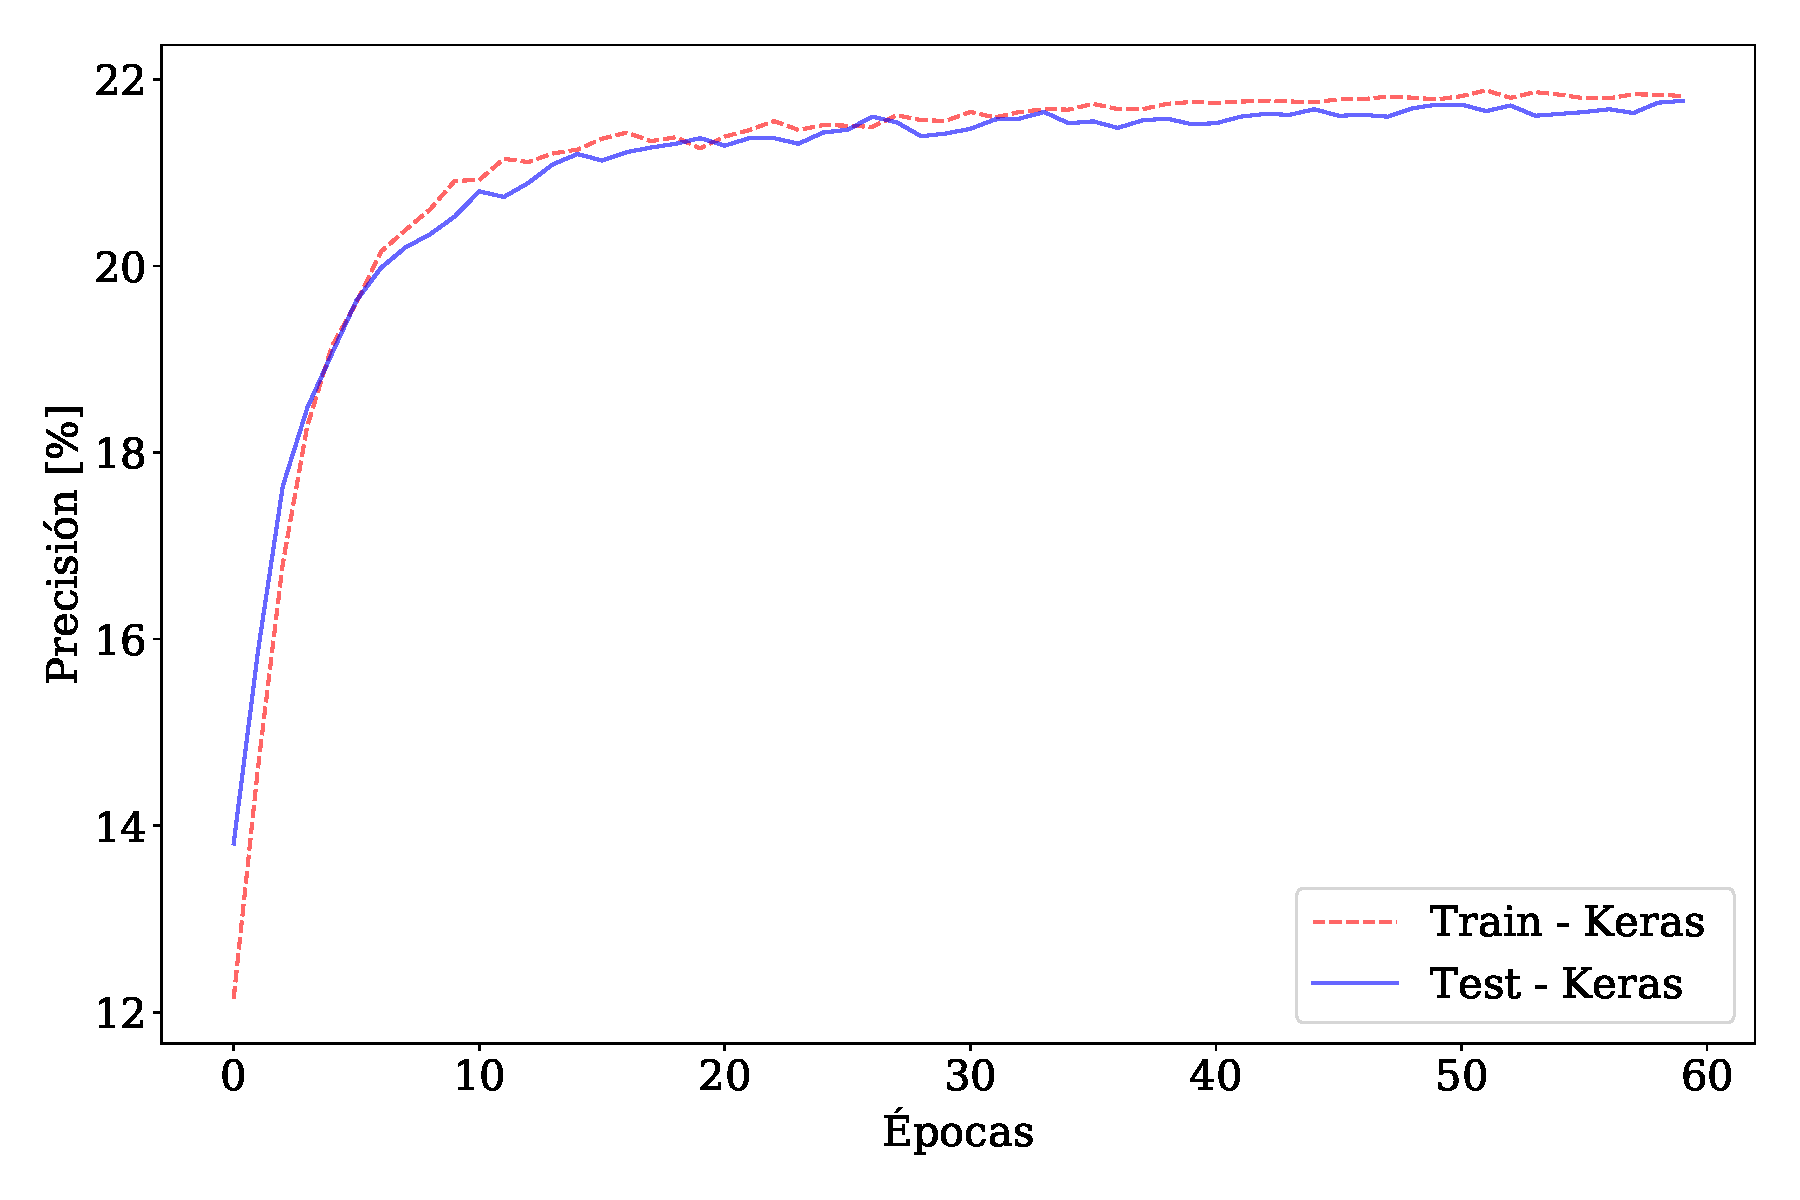
\includegraphics[width=0.5\textwidth]{Figs/ejer3_acc.pdf}
        \end{center}
        \caption{Precisión en función de las épocas}
        \label{fig:ejer3_acc}
    \end{small}
\end{figure}



\begin{figure}[H]
    \begin{small}
        \begin{center}
            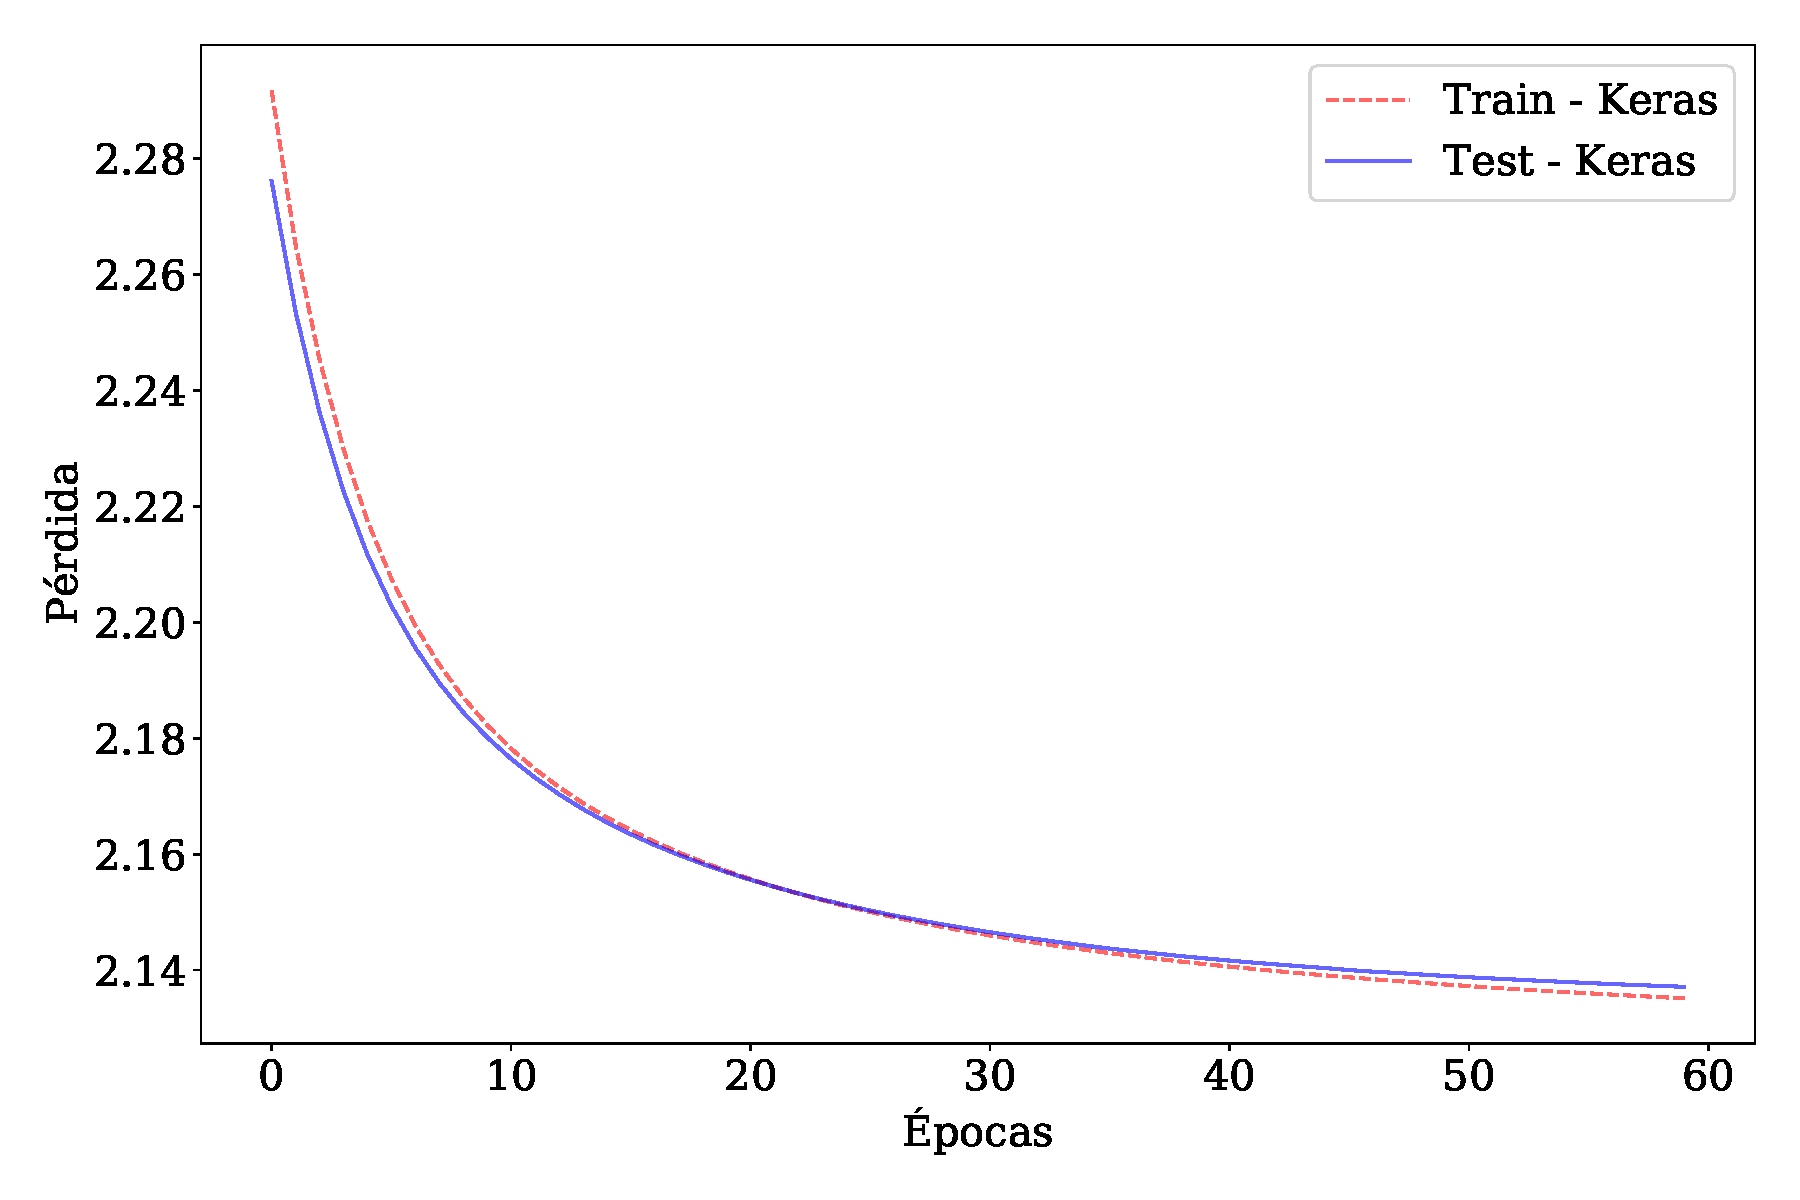
\includegraphics[width=0.5\textwidth]{Figs/ejer3_loss.pdf}
        \end{center}
        \caption{Pérdida en función de las épocas}
        \label{fig:ejer3_acc}
    \end{small}
\end{figure}


\section*{Ejercicio 4}
\emph{Utilizando los datos y la arquitectura que considere oportuna describir los distintos procesos para observar lo que la red neuronal ha aprendido.1}

\begin{figure}[H]
    \begin{small}
        \begin{center}
            
\includegraphics[width=0.25\textwidth]{Figs/random_init_img_epochs_50.pdf}
        \end{center}
        \caption{}
        \label{fig:random_init}
    \end{small}
\end{figure}


\begin{figure}[H]
    \begin{small}
        \begin{center}
            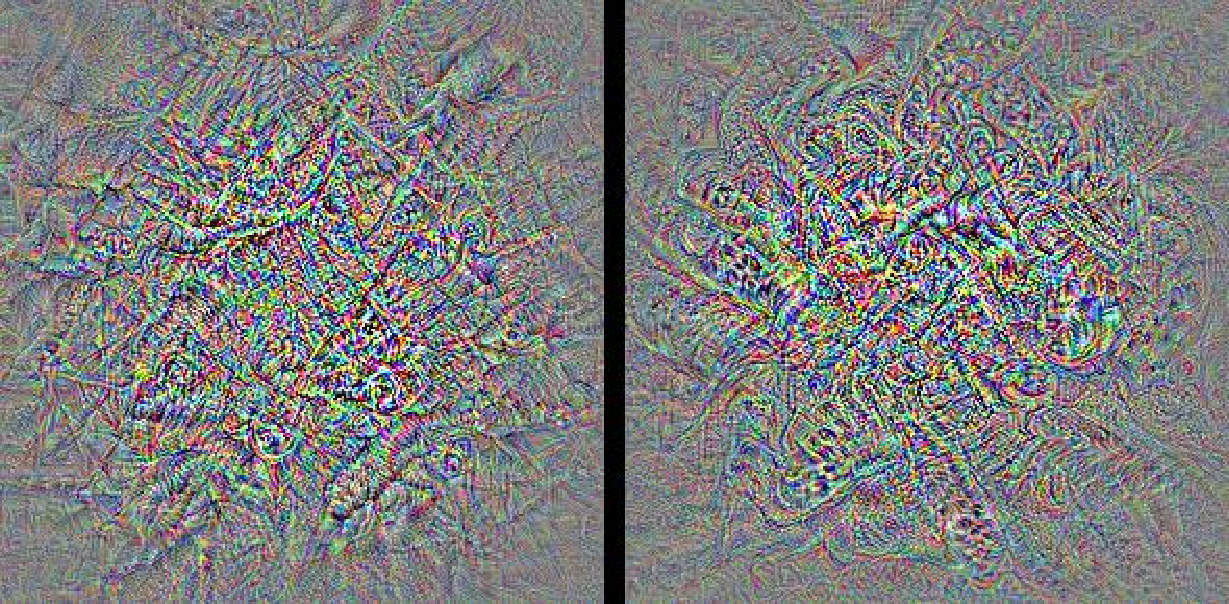
\includegraphics[width=0.5\textwidth]{Figs/random_filters_epochs_50.pdf}
        \end{center}
        \caption{}
        \label{fig:random_filters}
    \end{small}
\end{figure}

\begin{figure}[H]
    \begin{small}
        \begin{center}
            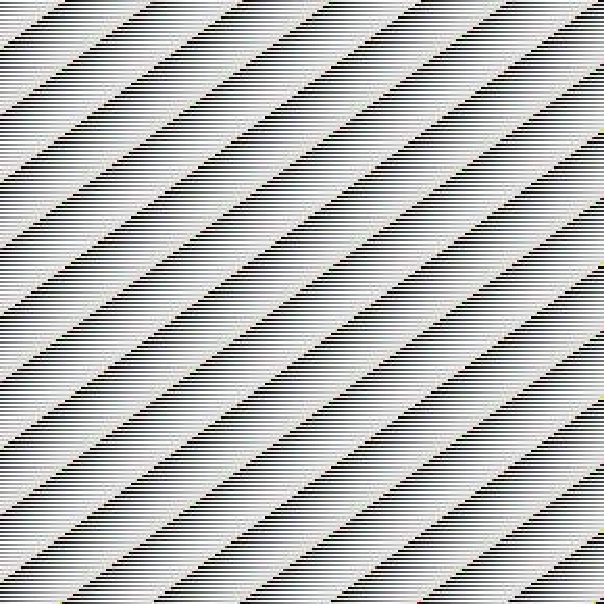
\includegraphics[width=0.25\textwidth]{Figs/sin_init_img_epochs_50.pdf}
        \end{center}
        \caption{}
        \label{fig:sin_init}
    \end{small}
\end{figure}



\begin{figure}[H]
    \begin{small}
        \begin{center}
            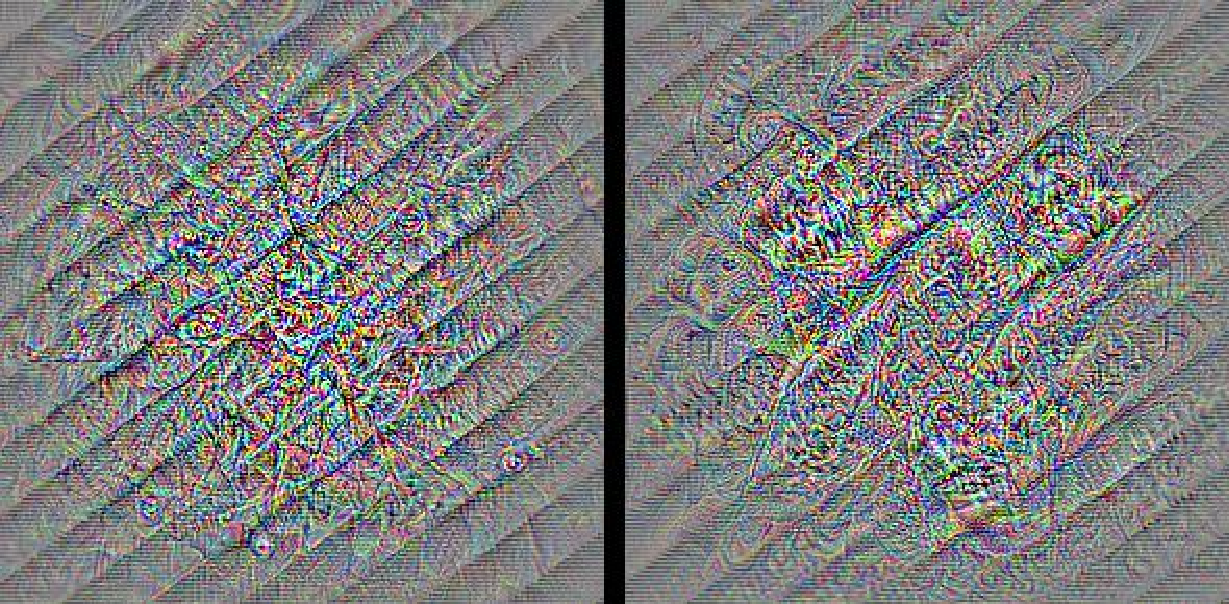
\includegraphics[width=0.5\textwidth]{Figs/sin_filters_epochs_50.pdf}
        \end{center}
        \caption{}
        \label{fig:sin_filters}
    \end{small}
\end{figure}

\begin{figure}[H]
    \begin{small}
        \begin{center}
            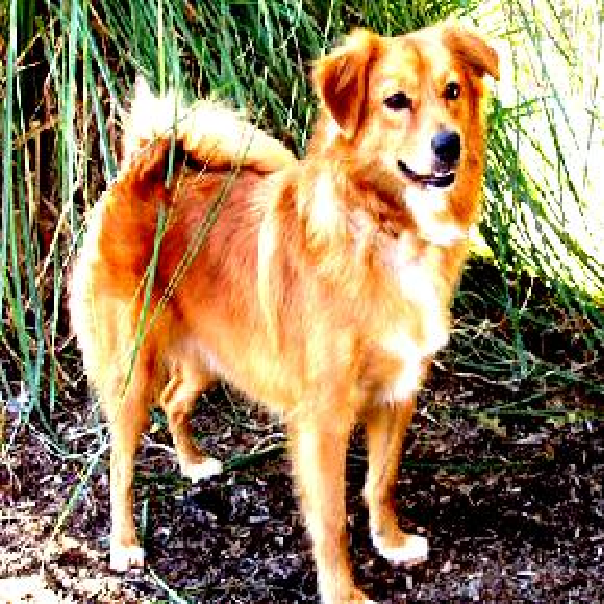
\includegraphics[width=0.25\textwidth]{Figs/perr2_init_img_epochs_50.pdf}
        \end{center}
        \caption{}
        \label{fig:perro_init}
    \end{small}
\end{figure}


\begin{figure}[H]
    \begin{small}
        \begin{center}
            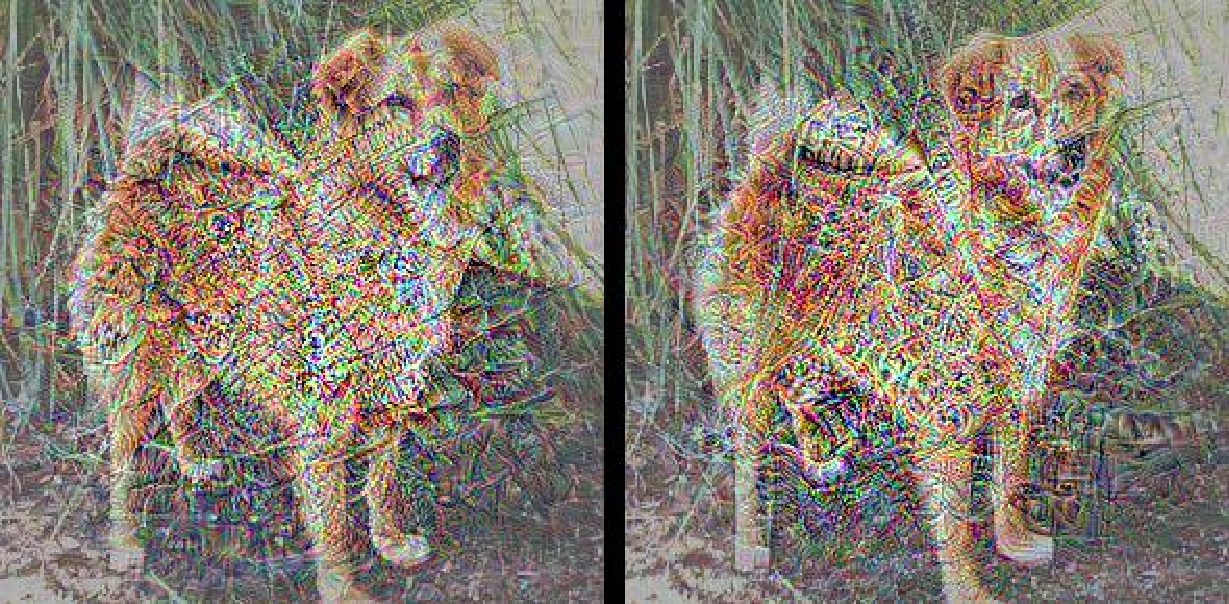
\includegraphics[width=0.5\textwidth]{Figs/perr2_filters_epochs_50.pdf}
        \end{center}
        \caption{}
        \label{fig:perro_filters}
    \end{small}
\end{figure}





\end{document}